\documentclass[12pt,a4paper]{article}
\usepackage[utf8]{inputenc}
\usepackage[english]{babel}
\usepackage{amsmath}
\usepackage{amsfonts}
\usepackage{amssymb}
\usepackage{graphicx}
\usepackage{hyperref}
\hypersetup{
    colorlinks=true,
    linkcolor=blue,
    filecolor=magenta,      
    urlcolor=cyan,
}
\usepackage[left=2cm,right=2cm,top=2cm,bottom=2cm]{geometry}
\author{Adrian Bach}
\title{Assessing visual representation of uncertainty in conservation policy makers-directed documents.}

\begin{document}
\maketitle

\tableofcontents

\vspace{\baselineskip}

Workshop title: "Engaging with uncertainty in natural research management and conservation: standards, perception, framing and decision making."

\section{Context \& Purpose}

Our group focuses on how readers interacts with the visual representation of scientific uncertainty (measures and model results).
A literature review around this topic was realized in order to eventually find a best practice for communicating this uncertainty to policy-makers in conservation.
In parallel to this, we thought it was interesting to assess the way uncertainty was currently visually represented in such documents.
Beside providing insights about the current habits in uncertainty communication in conservation, it will be interesting to confront the theory from the literature review to its actual application.
Was theory actually respected? If not, why was it not applied? Which kind of representation needs improvement?

%Workshop in NINA.
%Preliminary title "Communicating uncertainty from resource management models".\\
%Group 2: visual representation of uncertainty and users perception.
%Assessing the way uncertainty about scientific data (measures and models results) is currently represented in documents directed to conservation policy-makers.\\
For this figure review, I used the classification for visual representation of uncertainty provided in Kinkeldey et al. (2013).
In this study, around eighty papers about uncertainty representation in scientific papers were reviewed, allowing to identify five different levels of dichotomies:
\begin{itemize}
\item Explicit (uncertainty obtained from the data) / Implicit (displaying all the possibilities)
\item Extrinsic (new objects to represent uncertainty, \textit{e.g.} skewers, glyphs, intervals) / Intrinsic (altering the data visuals, \textit{e.g.} play on colors and shapes)
\item Visually integral (make sense only combined with the data) / Visually separable (still make sense when  separated from the data)
\item Coincident (represented in the same place as the data) / Adjacent (represented in another box than the data one's)
\item Static (inanimate figure) / Dynamic (interactive figure)
\end{itemize}
Based on these dichotomies, I characterized the way uncertainty was visually communicated in figures from a significant number of policy documents from different conservation organisations in order to produce a bar plot of the frequency of use of each representation combination.
%Beside giving a good idea of the current habits for uncertainty representation in conservation, it will also be interesting to compare the results with the best practice that will come out of the paper, and also target more accurately the areas of possible improvement.

\section{Methods}

The review was conduced by searching for conservation policy documents with an internet browser.
If the document found was relevant, and comprised a figure communicating scientific results, the methods were reviewed. %to assess if they involved any kind of uncertainty.
Any methods using means, medians or averages, measures on replicates, trend lines, estimates, computing model predictions, past and future estimations, different scenarios exploration, or compiled values from different studies, were considered eligible for representing data uncertainty.
If the methods involved one of these feature, the figure was classified using the categories from Kinkeldey et al. (2013).
When the same method produced several similar figures in single document, the uncertainty representation was assessed only once.
In a table (available on \href{https://github.com/AdrianBach/Workshop-task/blob/master/uncertrepres\textunderscore review2\textunderscore Rtreated.xlsx}{my GitHub}), a binary code was attributed (respectively 0 / 1 in the following categories) to if uncertainty representation was absent / present, explicit / implicit, extrinsic / intrinsic, visually integral / separable, coincident / adjacent, static / dynamic.
Additionally, the organisation, the focal natural feature, the type of figure (temporal, geographical, comparison, relationship, or pie chart), the year of production, the figure index, the criteria for uncertainty communication, as well as the URL address of the document were gathered in the same file.
A temporal figure is showing the evolution of a variable over time, a geographical figure is a spatially-explicit representation of the variation of a variable, and a comparison is a figure presenting values of a variable according to different categories (like bar plots or box-plots).

Currently, 47 visual representations of uncertainty were reviewed from figures in documents produced by the following organisations: European Environmental Council (EEA), Scottish National Heritage (SNH), Joint Nature Conservation Committee (JNCC), Australia's Convention on Biological Diversity (CBD), Intergovernmental Panel on Climate Change (IPCC), the Millennium Ecosystems Assessment, the Royal Society, the Food and Agriculture Organisation of the United Nations (FAO), the Department for Environment Food and Rural affairs of the United Kingdom, and the Intergovernmental Science-Policy Platform on Biodiversity and Ecosystem Services (IPBES), covering a publishing period ranging from 2003 to 2018.%\\
%For each figure in which uncertainty representation was relevant, gathered in a csv file the organisation, the focal natural feature, the year of production in text, for the first part.
%Then, attributed a binary code (respectively 0 / 1 in the following categories) to if uncertainty representation was absent / present, explicit / implicit, extrinsic / intrinsic, visually integral / separable, coincident / adjacent, static / dynamic.

The combination of binary information about each figure uncertainty representation was converted into a single binary number with a \href{https://github.com/AdrianBach/Workshop\textunderscore task/blob/master/bin2dec\textunderscore script.R}{custom R script} (\textit{e.g.} a representation of uncertainty being explicit, extrinsic, visually separable, coincident, and static would be 100100).
That way, each specific combination had a unique binary code, which was then converted into a unique decimal number for plotting convenience (same example, 100100 would be a 9).%\\
With the pivot chart tool on Excel, stacked bar plot displaying the counts of each combination was produced, along with a pie chart of the type of figure reviewed.

\section{First results}

\begin{figure}
\centering
\includegraphics[scale=0.5]{uncertainty_representation_review_figV2.pdf}
\caption{Frequency of use the different combinations of uncertainty representations from a 47 figures review of policy documents from different organizations. This is the representation I found the most useful for analysis, as it reveals some interesting patterns.}
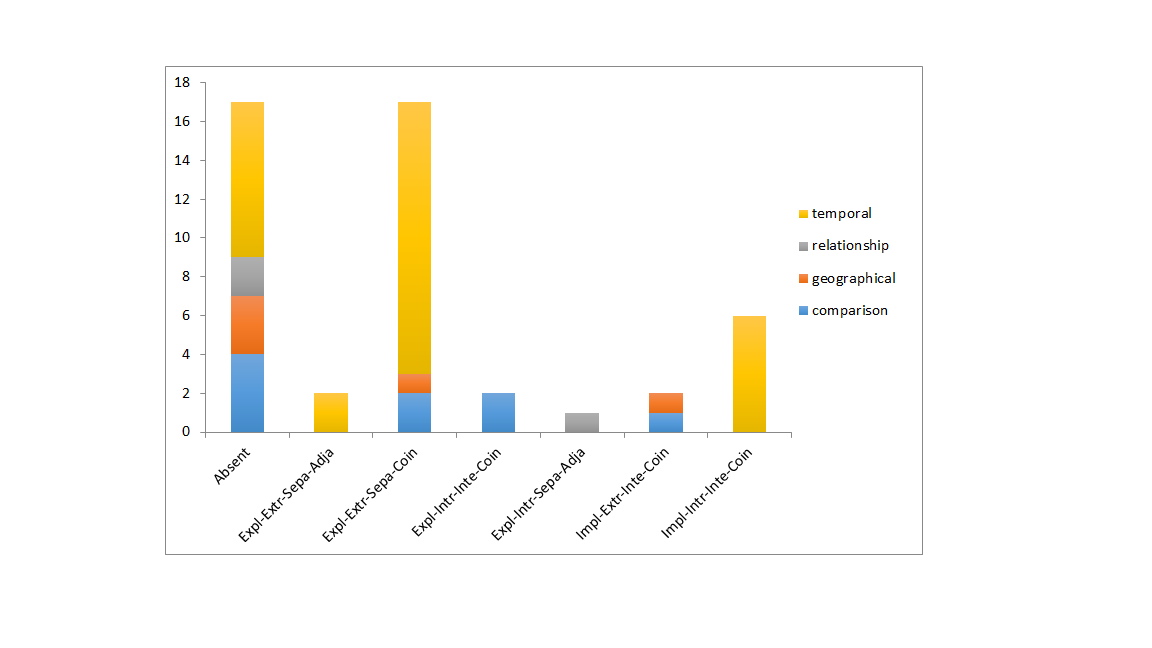
\includegraphics[scale=0.5]{workshop-figV2.png}
\caption{Alternative representation, hiding the combinations that were not observed in the review. I think the missing combinations are as informative as the present ones, but make the figure heavier.}
\label{res1}
\end{figure}
Firstly, uncertainty was not represented in 36\% (N = 47) of the reviewed figures, and
%When represented, only the explicit-extrinsic-visually separable combination has come out for now.\\
no Dynamic figure was seen yet.
Also, uncertainty was never represented in pie charts (for which color variations or shadings could be suitable?) in this sample.\\
Out of the figures in which uncertainty was communicated, more than half (17 out of 30) of the representations were Explicit, Intrinsic, visually Integral and Separable from the data, mostly in the form of standard deviation, confidence intervals, and error bars.\\
%Kinkeldey et al. (2013) suggested that it was unlikely that an Extrinsic representation of uncertainty would not as well be visually Separable from the data, which is verified here since such a combination was not observed.\\
The Implicit and visually Separable representation combination was also absent from this survey, most likely because with the Implicit representation, the uncertainty is communicated through the display of several different possibilities on the same figure, thus the information is lost if the representations are separated from one another.\\
It also comes out that a visually Integral representation cannot be Adjacent at the same time, which could be expected because if the representation does not make sense once separated from the data, it cannot be displayed aside without loosing the information.\\
%Why so many more Extr-Expl than Extr-Intr?
Finally, the survey show that the Explicit representations are more often Extrinsic than Intrinsic, could it be because adding on object on the data communicate uncertainty better than varying shapes or colors?
%Unexpectedly, uncertainty was not represented in any of the comparison figures, for which skewers are common practice in science.\\

\section{Elements of discussion}

%bias towards temporal figures
The fact that the survey plan is not balanced should be stressed here.
The number of examples is not the same for each type of figure, nor the number of examples per organizations.
Each organization can have particular practices, and if too many examples from the same organization are taken for the survey, it can induce a bias towards a certain practice, thus not being representative of the common practice.
Furthermore, 64\% of the figures reviewed being temporal (figure \ref{res2}), there might be another bias towards certain combinations here. 
Indeed, there might be representations that suits better particular combinations, for example it seems like Explicit - Extrinsic - Separable - Coincident representations are most commonly used for temporal figures.

\begin{figure}
\centering
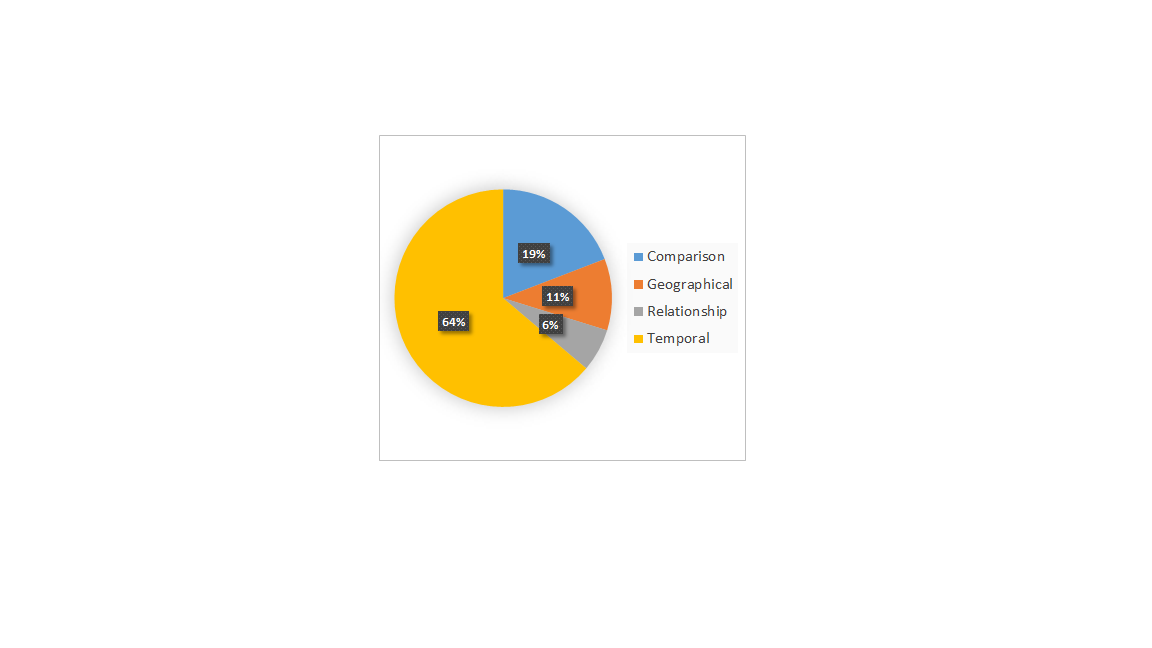
\includegraphics[scale=0.5]{workshop-figtype-piechart.png}
\caption{Proportion of each figure type in the review, showing the bias towards temporal figures.}
\label{res2}
\end{figure}


\end{document}